\documentclass[12pt]{article}
\usepackage[table]{xcolor}
\usepackage[shortlabels]{enumitem}
\usepackage{tabularx,xltabular}
\usepackage{graphicx}
\usepackage{hyperref}
\usepackage{verbatim}
\usepackage{geometry}
\usepackage{ulem}
\usepackage[official]{eurosym}
\usepackage{tikz}
\usetikzlibrary{arrows,backgrounds,calc,decorations.markings,patterns,3d}
\usepackage{pgfplots}
\pgfplotsset{compat = newest}
\usetikzlibrary{fit}
\newcommand\addvmargin[1]{
\usetikzlibrary{arrows}
\node[fit=(current bounding box),inner ysep=#1,inner xsep=0]{};}
\usepackage{cancel}
\usepackage{fontspec}
\usepackage{array}  
\geometry{a4paper, top=2cm, left=2cm, right=2cm, bottom=2cm, headsep=1cm}
\usepackage{tabu}
\usepackage{pst-node}
\usepackage{colortbl}
\usepackage{array}
\usepackage{german}
\setlength\parindent{0pt}
\newcolumntype{?}{!{\vrule width 1pt}}
\usepackage{makecell}
\renewcommand{\arraystretch}{2.5}
\usepackage{pbox}
\usepackage{amssymb}
\usepackage{amsmath}
\usepackage{booktabs}
\newcolumntype{L}[1]{>{\raggedright\let\newline\\\arraybackslash\hspace{0pt}}m{#1}}
\newcolumntype{C}[1]{>{\centering\let\newline\\\arraybackslash\hspace{0pt}}m{#1}}
\newcolumntype{R}[1]{>{\raggedleft\let\newline\\\arraybackslash\hspace{0pt}}m{#1}}
\begin{document}
\rightline{Datum: 08.06.2023}
\centerline{{\Large Tägliche Übungen}} 
\vspace{1cm}
\noindent \\


\begin{xltabular}{\textwidth}{|C{0.75cm}|X|C{0.75cm}|X|}
\arrayrulecolor{black}\hline
a)&$9\cdot x-18=45$
&
b)&$4\cdot b-12=12$
\\\hline
c)&$3\cdot y-6=6$
&
d)&$6\cdot b-12=12$
\\\hline
e)&$7\cdot a-10=32$
&
f)&$10\cdot b-18=12$
\\\hline
g)&$9\cdot x-19=35$
&
h)&$6\cdot y-15=3$
\\\hline
i)&$6\cdot b-14=22$
&
j)&$5\cdot y-10=0$
\\\hline
k)&$7\cdot b-3=67$
&
l)&$10\cdot b-8=22$
\\\hline
m)&$3\cdot x-9=9$
&
n)&$6\cdot y-8=46$
\\\hline
o)&$8\cdot y-6=10$
&
p)&$6\cdot y-19=-7$
\\\hline
q)&$4\cdot a-10=30$
&
r)&$4\cdot y-6=10$
\\\hline
s)&$2\cdot x-8=14$
&
t)&$9\cdot y-11=79$
\\\hline
u)&$6\cdot a-8=4$
&
v)&$6\cdot y-3=45$
\\\hline
w)&$5\cdot b-4=11$
&
x)&$2\cdot x-8=4$
\\\hline
y)&$5\cdot b-7=28$
&
z)&$8\cdot y-4=68$
\\\hline
\end{xltabular}
\vspace{0.5cm}
\newpage
\rightline{Datum: 08.06.2023}
\centerline{{\large Lösungen Tägliche Übungen}} 
\vspace{0.5cm}

\begin{xltabular}{\textwidth}{|C{0.75cm}|X|C{0.75cm}|X|}
\arrayrulecolor{black}\hline
a)&\begingroup\setlength{\jot}{-0.03cm}
\tikzstyle{background grid}=[draw, black!15,step=.5cm]
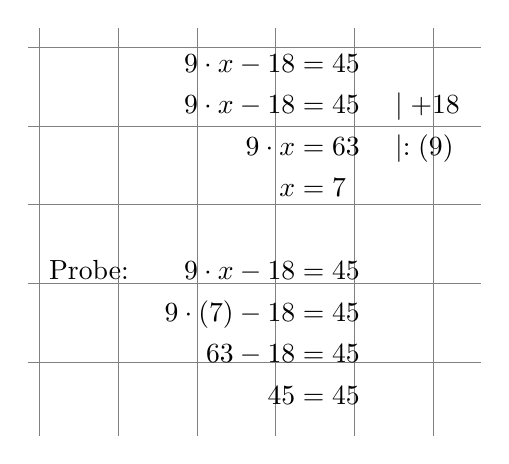
\begin{tikzpicture}[show background grid]
\node[below right] at (0,0.1) {
$\begin{aligned}
9\cdot x-18 &=45& &  \\
9\cdot x - 18 &=45& & \mid + 18\\
9\cdot x &=63& & \mid :\left(9\right)\\
x &=7& & 
\\
\\
\mbox{Probe:}\qquad 9\cdot x-18 &=45& &  \\
9\cdot \left(7\right)-18 &=45& &  \\
63-18 &=45& &  \\
45 &=45& &  \\
\end{aligned}$};
\end{tikzpicture}
\endgroup
&
b)&\begingroup\setlength{\jot}{-0.03cm}
\tikzstyle{background grid}=[draw, black!15,step=.5cm]
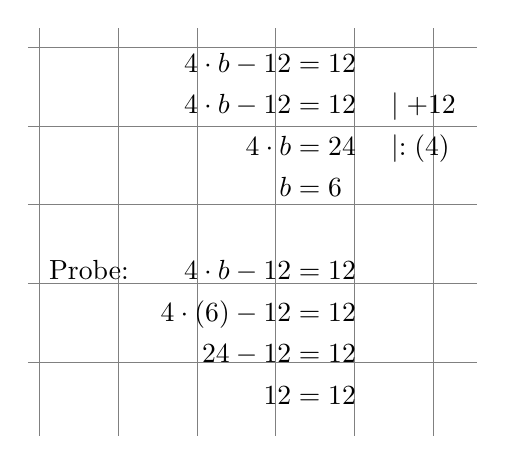
\begin{tikzpicture}[show background grid]
\node[below right] at (0,0.1) {
$\begin{aligned}
4\cdot b-12 &=12& &  \\
4\cdot b - 12 &=12& & \mid + 12\\
4\cdot b &=24& & \mid :\left(4\right)\\
b &=6& & 
\\
\\
\mbox{Probe:}\qquad 4\cdot b-12 &=12& &  \\
4\cdot \left(6\right)-12 &=12& &  \\
24-12 &=12& &  \\
12 &=12& &  \\
\end{aligned}$};
\end{tikzpicture}
\endgroup
\\\hline
c)&\begingroup\setlength{\jot}{-0.03cm}
\tikzstyle{background grid}=[draw, black!15,step=.5cm]
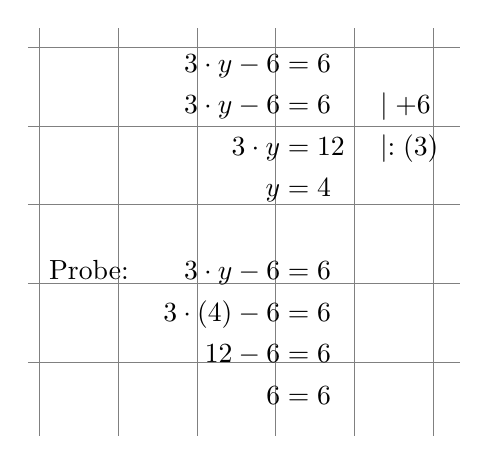
\begin{tikzpicture}[show background grid]
\node[below right] at (0,0.1) {
$\begin{aligned}
3\cdot y-6 &=6& &  \\
3\cdot y - 6 &=6& & \mid + 6\\
3\cdot y &=12& & \mid :\left(3\right)\\
y &=4& & 
\\
\\
\mbox{Probe:}\qquad 3\cdot y-6 &=6& &  \\
3\cdot \left(4\right)-6 &=6& &  \\
12-6 &=6& &  \\
6 &=6& &  \\
\end{aligned}$};
\end{tikzpicture}
\endgroup
&
d)&\begingroup\setlength{\jot}{-0.03cm}
\tikzstyle{background grid}=[draw, black!15,step=.5cm]
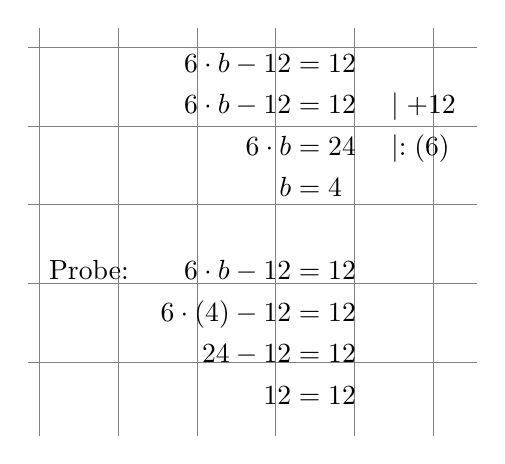
\begin{tikzpicture}[show background grid]
\node[below right] at (0,0.1) {
$\begin{aligned}
6\cdot b-12 &=12& &  \\
6\cdot b - 12 &=12& & \mid + 12\\
6\cdot b &=24& & \mid :\left(6\right)\\
b &=4& & 
\\
\\
\mbox{Probe:}\qquad 6\cdot b-12 &=12& &  \\
6\cdot \left(4\right)-12 &=12& &  \\
24-12 &=12& &  \\
12 &=12& &  \\
\end{aligned}$};
\end{tikzpicture}
\endgroup
\\\hline
e)&\begingroup\setlength{\jot}{-0.03cm}
\tikzstyle{background grid}=[draw, black!15,step=.5cm]
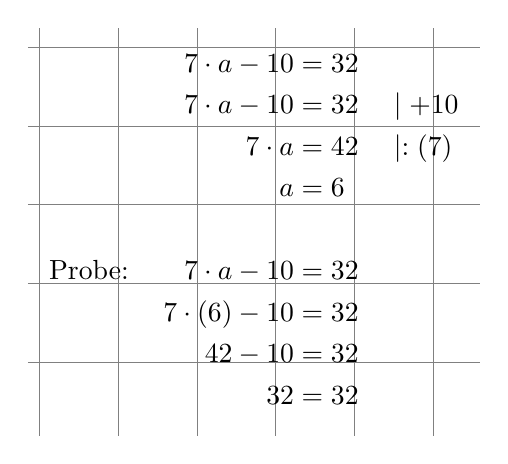
\begin{tikzpicture}[show background grid]
\node[below right] at (0,0.1) {
$\begin{aligned}
7\cdot a-10 &=32& &  \\
7\cdot a - 10 &=32& & \mid + 10\\
7\cdot a &=42& & \mid :\left(7\right)\\
a &=6& & 
\\
\\
\mbox{Probe:}\qquad 7\cdot a-10 &=32& &  \\
7\cdot \left(6\right)-10 &=32& &  \\
42-10 &=32& &  \\
32 &=32& &  \\
\end{aligned}$};
\end{tikzpicture}
\endgroup
&
f)&\begingroup\setlength{\jot}{-0.03cm}
\tikzstyle{background grid}=[draw, black!15,step=.5cm]
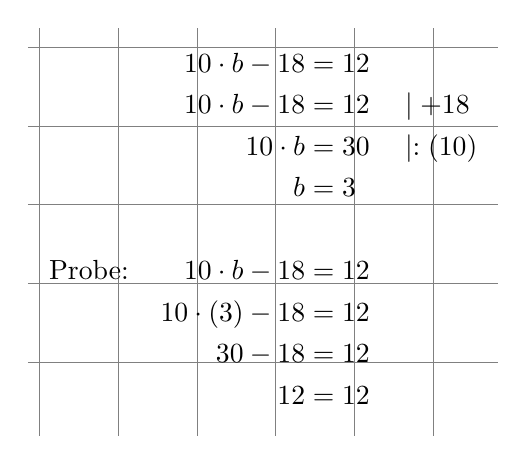
\begin{tikzpicture}[show background grid]
\node[below right] at (0,0.1) {
$\begin{aligned}
10\cdot b-18 &=12& &  \\
10\cdot b - 18 &=12& & \mid + 18\\
10\cdot b &=30& & \mid :\left(10\right)\\
b &=3& & 
\\
\\
\mbox{Probe:}\qquad 10\cdot b-18 &=12& &  \\
10\cdot \left(3\right)-18 &=12& &  \\
30-18 &=12& &  \\
12 &=12& &  \\
\end{aligned}$};
\end{tikzpicture}
\endgroup
\\\hline
g)&\begingroup\setlength{\jot}{-0.03cm}
\tikzstyle{background grid}=[draw, black!15,step=.5cm]
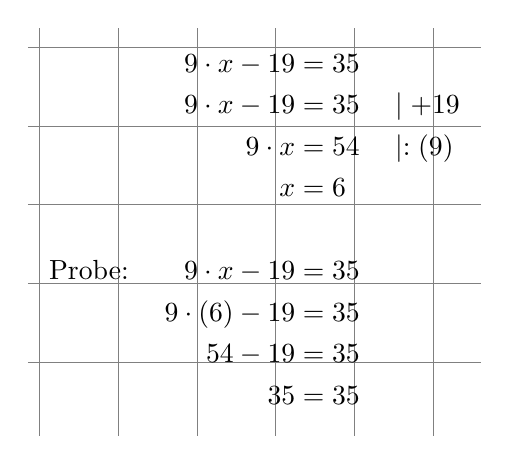
\begin{tikzpicture}[show background grid]
\node[below right] at (0,0.1) {
$\begin{aligned}
9\cdot x-19 &=35& &  \\
9\cdot x - 19 &=35& & \mid + 19\\
9\cdot x &=54& & \mid :\left(9\right)\\
x &=6& & 
\\
\\
\mbox{Probe:}\qquad 9\cdot x-19 &=35& &  \\
9\cdot \left(6\right)-19 &=35& &  \\
54-19 &=35& &  \\
35 &=35& &  \\
\end{aligned}$};
\end{tikzpicture}
\endgroup
&
h)&\begingroup\setlength{\jot}{-0.03cm}
\tikzstyle{background grid}=[draw, black!15,step=.5cm]
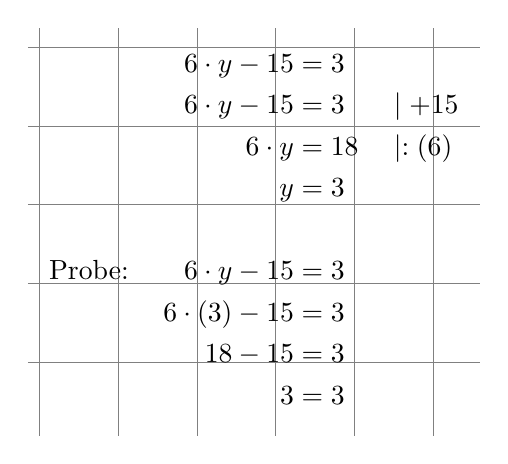
\begin{tikzpicture}[show background grid]
\node[below right] at (0,0.1) {
$\begin{aligned}
6\cdot y-15 &=3& &  \\
6\cdot y - 15 &=3& & \mid + 15\\
6\cdot y &=18& & \mid :\left(6\right)\\
y &=3& & 
\\
\\
\mbox{Probe:}\qquad 6\cdot y-15 &=3& &  \\
6\cdot \left(3\right)-15 &=3& &  \\
18-15 &=3& &  \\
3 &=3& &  \\
\end{aligned}$};
\end{tikzpicture}
\endgroup
\\\hline
i)&\begingroup\setlength{\jot}{-0.03cm}
\tikzstyle{background grid}=[draw, black!15,step=.5cm]
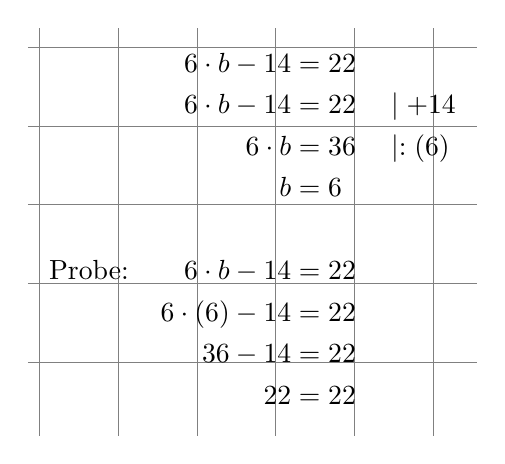
\begin{tikzpicture}[show background grid]
\node[below right] at (0,0.1) {
$\begin{aligned}
6\cdot b-14 &=22& &  \\
6\cdot b - 14 &=22& & \mid + 14\\
6\cdot b &=36& & \mid :\left(6\right)\\
b &=6& & 
\\
\\
\mbox{Probe:}\qquad 6\cdot b-14 &=22& &  \\
6\cdot \left(6\right)-14 &=22& &  \\
36-14 &=22& &  \\
22 &=22& &  \\
\end{aligned}$};
\end{tikzpicture}
\endgroup
&
j)&\begingroup\setlength{\jot}{-0.03cm}
\tikzstyle{background grid}=[draw, black!15,step=.5cm]
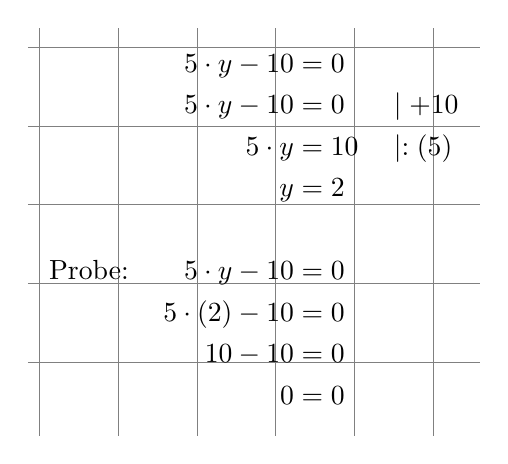
\begin{tikzpicture}[show background grid]
\node[below right] at (0,0.1) {
$\begin{aligned}
5\cdot y-10 &=0& &  \\
5\cdot y - 10 &=0& & \mid + 10\\
5\cdot y &=10& & \mid :\left(5\right)\\
y &=2& & 
\\
\\
\mbox{Probe:}\qquad 5\cdot y-10 &=0& &  \\
5\cdot \left(2\right)-10 &=0& &  \\
10-10 &=0& &  \\
0 &=0& &  \\
\end{aligned}$};
\end{tikzpicture}
\endgroup
\\\hline
k)&\begingroup\setlength{\jot}{-0.03cm}
\tikzstyle{background grid}=[draw, black!15,step=.5cm]
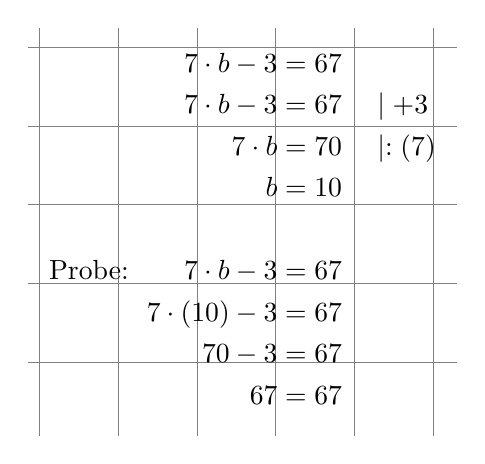
\begin{tikzpicture}[show background grid]
\node[below right] at (0,0.1) {
$\begin{aligned}
7\cdot b-3 &=67& &  \\
7\cdot b - 3 &=67& & \mid + 3\\
7\cdot b &=70& & \mid :\left(7\right)\\
b &=10& & 
\\
\\
\mbox{Probe:}\qquad 7\cdot b-3 &=67& &  \\
7\cdot \left(10\right)-3 &=67& &  \\
70-3 &=67& &  \\
67 &=67& &  \\
\end{aligned}$};
\end{tikzpicture}
\endgroup
&
l)&\begingroup\setlength{\jot}{-0.03cm}
\tikzstyle{background grid}=[draw, black!15,step=.5cm]
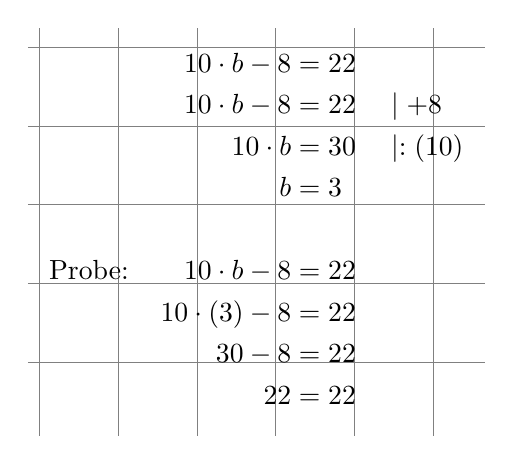
\begin{tikzpicture}[show background grid]
\node[below right] at (0,0.1) {
$\begin{aligned}
10\cdot b-8 &=22& &  \\
10\cdot b - 8 &=22& & \mid + 8\\
10\cdot b &=30& & \mid :\left(10\right)\\
b &=3& & 
\\
\\
\mbox{Probe:}\qquad 10\cdot b-8 &=22& &  \\
10\cdot \left(3\right)-8 &=22& &  \\
30-8 &=22& &  \\
22 &=22& &  \\
\end{aligned}$};
\end{tikzpicture}
\endgroup
\\\hline
m)&\begingroup\setlength{\jot}{-0.03cm}
\tikzstyle{background grid}=[draw, black!15,step=.5cm]
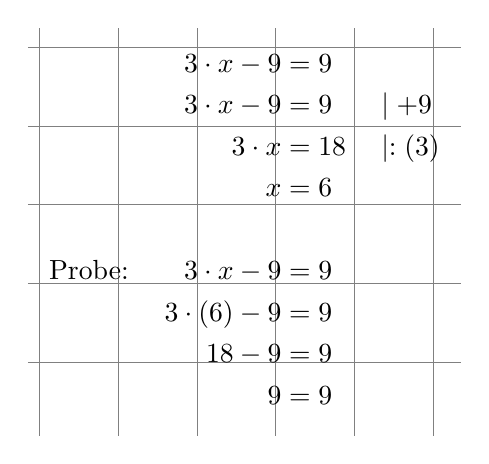
\begin{tikzpicture}[show background grid]
\node[below right] at (0,0.1) {
$\begin{aligned}
3\cdot x-9 &=9& &  \\
3\cdot x - 9 &=9& & \mid + 9\\
3\cdot x &=18& & \mid :\left(3\right)\\
x &=6& & 
\\
\\
\mbox{Probe:}\qquad 3\cdot x-9 &=9& &  \\
3\cdot \left(6\right)-9 &=9& &  \\
18-9 &=9& &  \\
9 &=9& &  \\
\end{aligned}$};
\end{tikzpicture}
\endgroup
&
n)&\begingroup\setlength{\jot}{-0.03cm}
\tikzstyle{background grid}=[draw, black!15,step=.5cm]
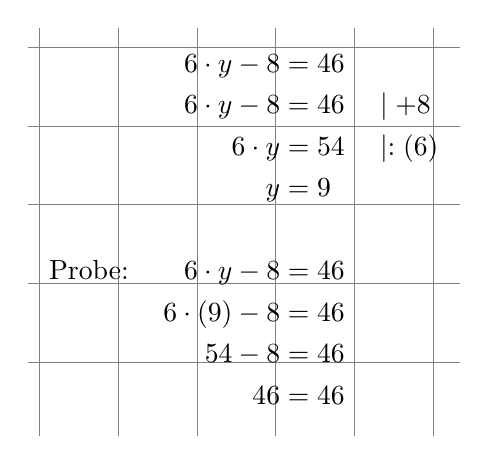
\begin{tikzpicture}[show background grid]
\node[below right] at (0,0.1) {
$\begin{aligned}
6\cdot y-8 &=46& &  \\
6\cdot y - 8 &=46& & \mid + 8\\
6\cdot y &=54& & \mid :\left(6\right)\\
y &=9& & 
\\
\\
\mbox{Probe:}\qquad 6\cdot y-8 &=46& &  \\
6\cdot \left(9\right)-8 &=46& &  \\
54-8 &=46& &  \\
46 &=46& &  \\
\end{aligned}$};
\end{tikzpicture}
\endgroup
\\\hline
o)&\begingroup\setlength{\jot}{-0.03cm}
\tikzstyle{background grid}=[draw, black!15,step=.5cm]
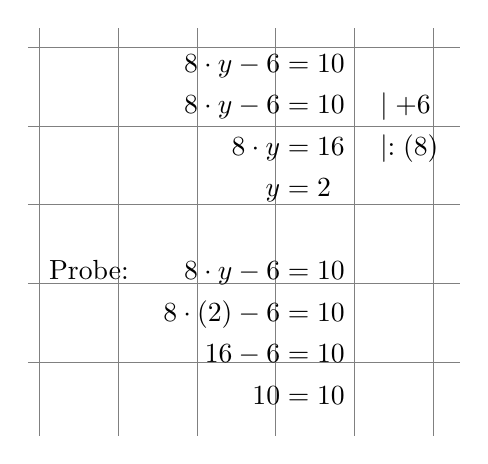
\begin{tikzpicture}[show background grid]
\node[below right] at (0,0.1) {
$\begin{aligned}
8\cdot y-6 &=10& &  \\
8\cdot y - 6 &=10& & \mid + 6\\
8\cdot y &=16& & \mid :\left(8\right)\\
y &=2& & 
\\
\\
\mbox{Probe:}\qquad 8\cdot y-6 &=10& &  \\
8\cdot \left(2\right)-6 &=10& &  \\
16-6 &=10& &  \\
10 &=10& &  \\
\end{aligned}$};
\end{tikzpicture}
\endgroup
&
p)&\begingroup\setlength{\jot}{-0.03cm}
\tikzstyle{background grid}=[draw, black!15,step=.5cm]
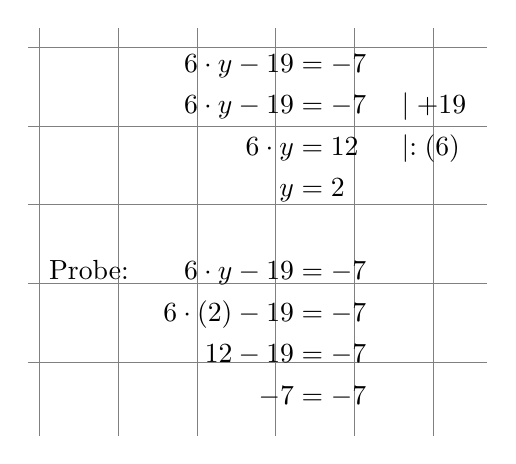
\begin{tikzpicture}[show background grid]
\node[below right] at (0,0.1) {
$\begin{aligned}
6\cdot y-19 &=-7& &  \\
6\cdot y - 19 &=-7& & \mid + 19\\
6\cdot y &=12& & \mid :\left(6\right)\\
y &=2& & 
\\
\\
\mbox{Probe:}\qquad 6\cdot y-19 &=-7& &  \\
6\cdot \left(2\right)-19 &=-7& &  \\
12-19 &=-7& &  \\
-7 &=-7& &  \\
\end{aligned}$};
\end{tikzpicture}
\endgroup
\\\hline
q)&\begingroup\setlength{\jot}{-0.03cm}
\tikzstyle{background grid}=[draw, black!15,step=.5cm]
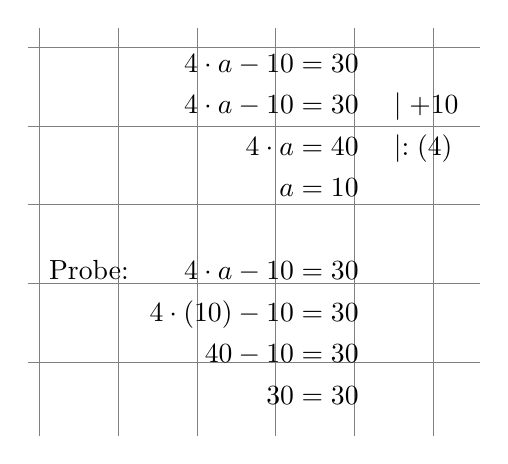
\begin{tikzpicture}[show background grid]
\node[below right] at (0,0.1) {
$\begin{aligned}
4\cdot a-10 &=30& &  \\
4\cdot a - 10 &=30& & \mid + 10\\
4\cdot a &=40& & \mid :\left(4\right)\\
a &=10& & 
\\
\\
\mbox{Probe:}\qquad 4\cdot a-10 &=30& &  \\
4\cdot \left(10\right)-10 &=30& &  \\
40-10 &=30& &  \\
30 &=30& &  \\
\end{aligned}$};
\end{tikzpicture}
\endgroup
&
r)&\begingroup\setlength{\jot}{-0.03cm}
\tikzstyle{background grid}=[draw, black!15,step=.5cm]
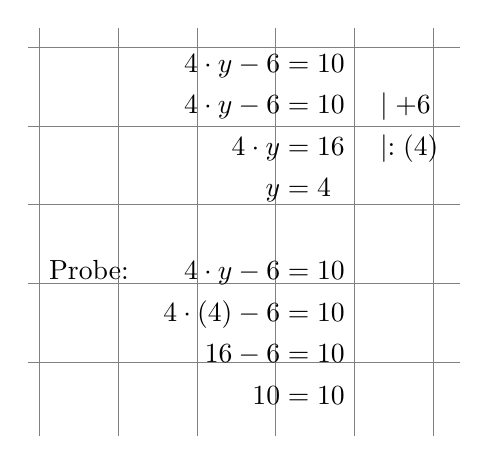
\begin{tikzpicture}[show background grid]
\node[below right] at (0,0.1) {
$\begin{aligned}
4\cdot y-6 &=10& &  \\
4\cdot y - 6 &=10& & \mid + 6\\
4\cdot y &=16& & \mid :\left(4\right)\\
y &=4& & 
\\
\\
\mbox{Probe:}\qquad 4\cdot y-6 &=10& &  \\
4\cdot \left(4\right)-6 &=10& &  \\
16-6 &=10& &  \\
10 &=10& &  \\
\end{aligned}$};
\end{tikzpicture}
\endgroup
\\\hline
s)&\begingroup\setlength{\jot}{-0.03cm}
\tikzstyle{background grid}=[draw, black!15,step=.5cm]
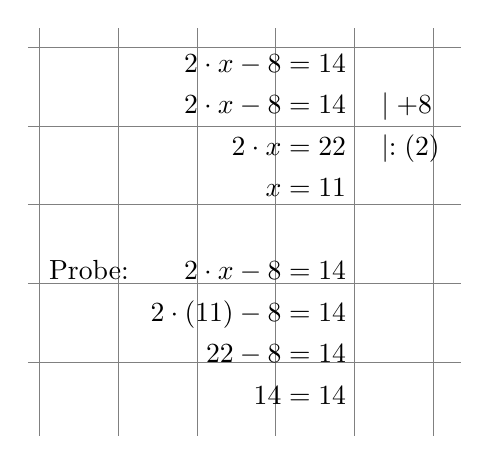
\begin{tikzpicture}[show background grid]
\node[below right] at (0,0.1) {
$\begin{aligned}
2\cdot x-8 &=14& &  \\
2\cdot x - 8 &=14& & \mid + 8\\
2\cdot x &=22& & \mid :\left(2\right)\\
x &=11& & 
\\
\\
\mbox{Probe:}\qquad 2\cdot x-8 &=14& &  \\
2\cdot \left(11\right)-8 &=14& &  \\
22-8 &=14& &  \\
14 &=14& &  \\
\end{aligned}$};
\end{tikzpicture}
\endgroup
&
t)&\begingroup\setlength{\jot}{-0.03cm}
\tikzstyle{background grid}=[draw, black!15,step=.5cm]
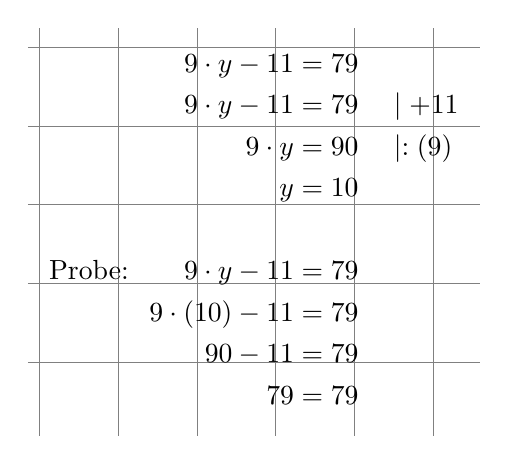
\begin{tikzpicture}[show background grid]
\node[below right] at (0,0.1) {
$\begin{aligned}
9\cdot y-11 &=79& &  \\
9\cdot y - 11 &=79& & \mid + 11\\
9\cdot y &=90& & \mid :\left(9\right)\\
y &=10& & 
\\
\\
\mbox{Probe:}\qquad 9\cdot y-11 &=79& &  \\
9\cdot \left(10\right)-11 &=79& &  \\
90-11 &=79& &  \\
79 &=79& &  \\
\end{aligned}$};
\end{tikzpicture}
\endgroup
\\\hline
u)&\begingroup\setlength{\jot}{-0.03cm}
\tikzstyle{background grid}=[draw, black!15,step=.5cm]
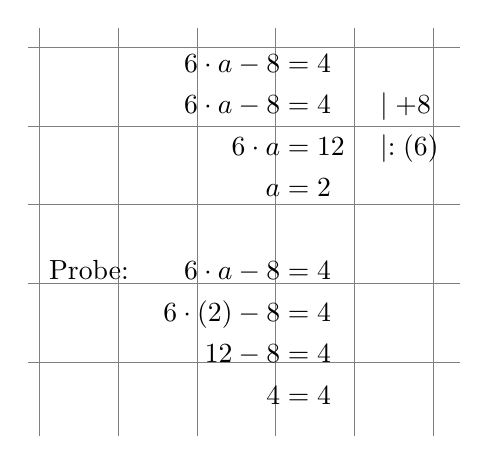
\begin{tikzpicture}[show background grid]
\node[below right] at (0,0.1) {
$\begin{aligned}
6\cdot a-8 &=4& &  \\
6\cdot a - 8 &=4& & \mid + 8\\
6\cdot a &=12& & \mid :\left(6\right)\\
a &=2& & 
\\
\\
\mbox{Probe:}\qquad 6\cdot a-8 &=4& &  \\
6\cdot \left(2\right)-8 &=4& &  \\
12-8 &=4& &  \\
4 &=4& &  \\
\end{aligned}$};
\end{tikzpicture}
\endgroup
&
v)&\begingroup\setlength{\jot}{-0.03cm}
\tikzstyle{background grid}=[draw, black!15,step=.5cm]
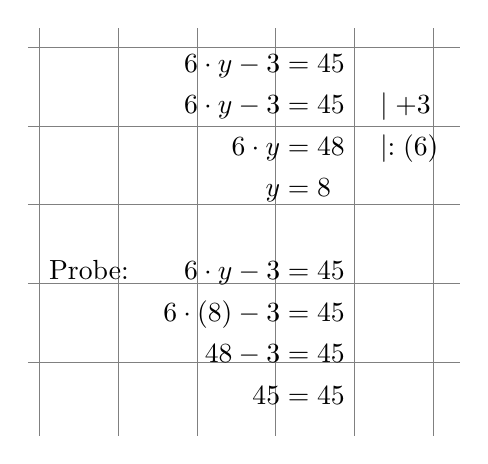
\begin{tikzpicture}[show background grid]
\node[below right] at (0,0.1) {
$\begin{aligned}
6\cdot y-3 &=45& &  \\
6\cdot y - 3 &=45& & \mid + 3\\
6\cdot y &=48& & \mid :\left(6\right)\\
y &=8& & 
\\
\\
\mbox{Probe:}\qquad 6\cdot y-3 &=45& &  \\
6\cdot \left(8\right)-3 &=45& &  \\
48-3 &=45& &  \\
45 &=45& &  \\
\end{aligned}$};
\end{tikzpicture}
\endgroup
\\\hline
w)&\begingroup\setlength{\jot}{-0.03cm}
\tikzstyle{background grid}=[draw, black!15,step=.5cm]
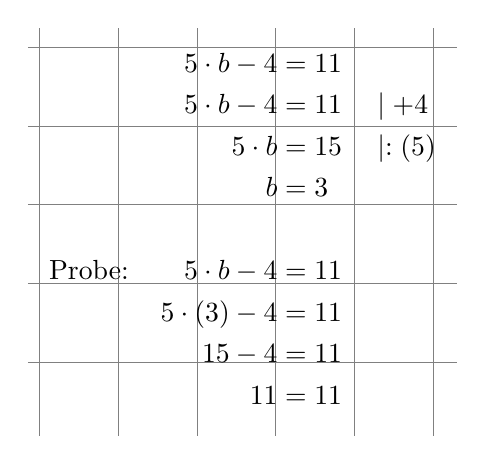
\begin{tikzpicture}[show background grid]
\node[below right] at (0,0.1) {
$\begin{aligned}
5\cdot b-4 &=11& &  \\
5\cdot b - 4 &=11& & \mid + 4\\
5\cdot b &=15& & \mid :\left(5\right)\\
b &=3& & 
\\
\\
\mbox{Probe:}\qquad 5\cdot b-4 &=11& &  \\
5\cdot \left(3\right)-4 &=11& &  \\
15-4 &=11& &  \\
11 &=11& &  \\
\end{aligned}$};
\end{tikzpicture}
\endgroup
&
x)&\begingroup\setlength{\jot}{-0.03cm}
\tikzstyle{background grid}=[draw, black!15,step=.5cm]
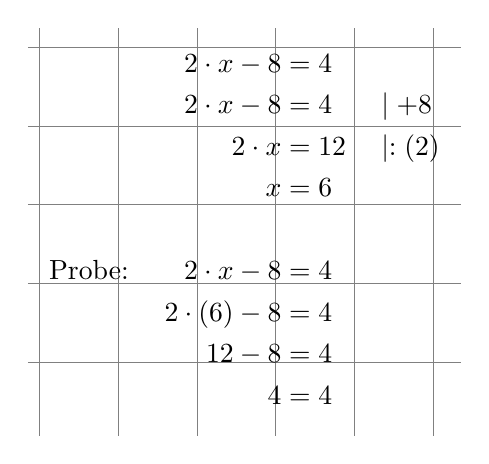
\begin{tikzpicture}[show background grid]
\node[below right] at (0,0.1) {
$\begin{aligned}
2\cdot x-8 &=4& &  \\
2\cdot x - 8 &=4& & \mid + 8\\
2\cdot x &=12& & \mid :\left(2\right)\\
x &=6& & 
\\
\\
\mbox{Probe:}\qquad 2\cdot x-8 &=4& &  \\
2\cdot \left(6\right)-8 &=4& &  \\
12-8 &=4& &  \\
4 &=4& &  \\
\end{aligned}$};
\end{tikzpicture}
\endgroup
\\\hline
y)&\begingroup\setlength{\jot}{-0.03cm}
\tikzstyle{background grid}=[draw, black!15,step=.5cm]
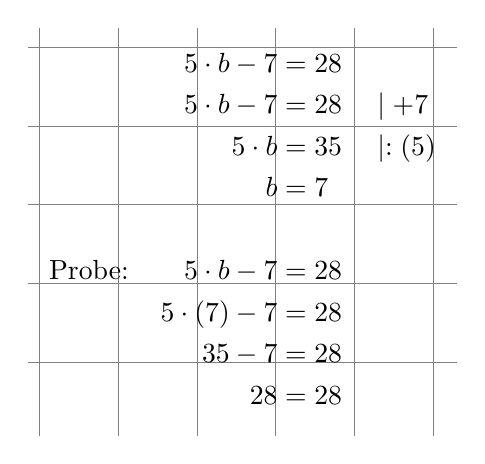
\begin{tikzpicture}[show background grid]
\node[below right] at (0,0.1) {
$\begin{aligned}
5\cdot b-7 &=28& &  \\
5\cdot b - 7 &=28& & \mid + 7\\
5\cdot b &=35& & \mid :\left(5\right)\\
b &=7& & 
\\
\\
\mbox{Probe:}\qquad 5\cdot b-7 &=28& &  \\
5\cdot \left(7\right)-7 &=28& &  \\
35-7 &=28& &  \\
28 &=28& &  \\
\end{aligned}$};
\end{tikzpicture}
\endgroup
&
z)&\begingroup\setlength{\jot}{-0.03cm}
\tikzstyle{background grid}=[draw, black!15,step=.5cm]
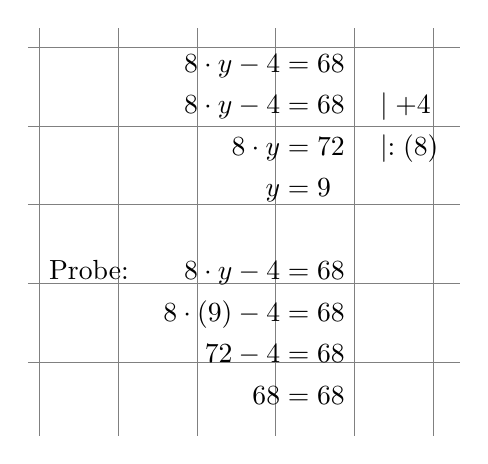
\begin{tikzpicture}[show background grid]
\node[below right] at (0,0.1) {
$\begin{aligned}
8\cdot y-4 &=68& &  \\
8\cdot y - 4 &=68& & \mid + 4\\
8\cdot y &=72& & \mid :\left(8\right)\\
y &=9& & 
\\
\\
\mbox{Probe:}\qquad 8\cdot y-4 &=68& &  \\
8\cdot \left(9\right)-4 &=68& &  \\
72-4 &=68& &  \\
68 &=68& &  \\
\end{aligned}$};
\end{tikzpicture}
\endgroup
\\\hline
\end{xltabular}
\vspace{0.5cm}
\end{document}